\documentclass[border=6pt]{standalone}
\usepackage{tikz}
\usetikzlibrary{arrows.meta}
\begin{document}
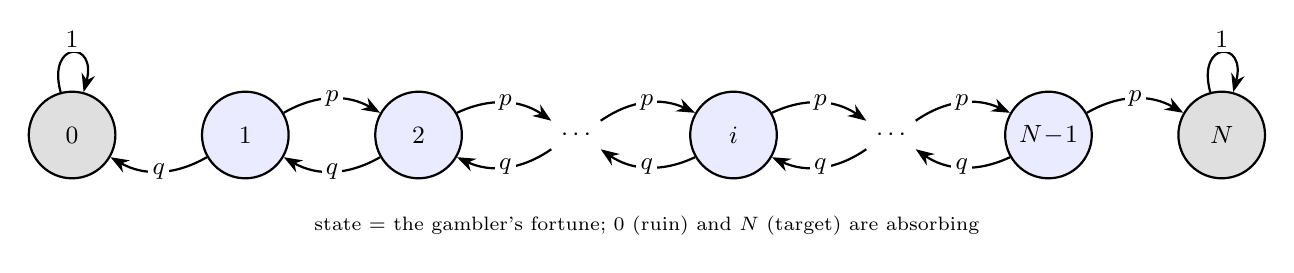
\begin{tikzpicture}[>=Stealth,font=\small,
 s/.style={draw,thick,circle,minimum size=1.1cm,inner sep=0pt,fill=blue!8},
 e/.style={->,thick},
 lab/.style={font=\small,fill=white,inner sep=1.5pt},
 every loop/.style={->,thick,looseness=6}]
\node[s,fill=gray!25] (0) at (0,0) {$0$};
\node[s] (1) at (2.2,0) {$1$};
\node[s] (2) at (4.4,0) {$2$};
\node (d) at (6.4,0) {$\cdots$};
\node[s] (i) at (8.4,0) {$i$};
\node (d2) at (10.4,0) {$\cdots$};
\node[s] (N1) at (12.4,0) {$N\!-\!1$};
\node[s,fill=gray!25] (N) at (14.6,0) {$N$};
\foreach \a/\b in {1/2,2/d,d/i,i/d2,d2/N1,N1/N} \draw[e] (\a) to[bend left=30] node[lab]{$p$} (\b);
\foreach \a/\b in {1/0,2/1,d/2,i/d,d2/i,N1/d2} \draw[e] (\a) to[bend left=30] node[lab]{$q$} (\b);
\path (0) edge[loop above] node[lab]{1} (0);
\path (N) edge[loop above] node[lab]{1} (N);
\node[font=\scriptsize,align=center] at (7.3,-1.15) {state = the gambler's fortune; $0$ (ruin) and $N$ (target) are absorbing};
\end{tikzpicture}
\end{document}
